%%%%%%%%%%%%%%%%%%%%%%%%%%%%%%%%%%%%%%%%%
% Beamer Presentation
% LaTeX Template
% Version 1.0 (10/11/12)
%
% This template has been downloaded from:
% http://www.LaTeXTemplates.com
%
% License:
% CC BY-NC-SA 3.0 (http://creativecommons.org/licenses/by-nc-sa/3.0/)
%
%%%%%%%%%%%%%%%%%%%%%%%%%%%%%%%%%%%%%%%%%

%----------------------------------------------------------------------------------------
%	PACKAGES AND THEMES
%----------------------------------------------------------------------------------------

%\documentclass[UTF8,aspectratio=169,14pt]{ctexbeamer}
\documentclass[UTF8,aspectratio=169]{ctexbeamer}
\usepackage{hyperref}
\hypersetup{
	colorlinks=true,
	linkcolor=red,
	anchorcolor=blue,
	citecolor=green
}

\mode<presentation> {
	
	% The Beamer class comes with a number of default slide themes
	% which change the colors and layouts of slides. Below this is a list
	% of all the themes, uncomment each in turn to see what they look like.
	
	%\usetheme{default}
	%\usetheme{AnnArbor}
	%\usetheme{Antibes}
	%\usetheme{Bergen}
	%\usetheme{Berkeley}
	%\usetheme{Berlin}
	%\usetheme{Boadilla}
	%\usetheme{CambridgeUS}
	%\usetheme{Copenhagen}
	%\usetheme{Darmstadt}
	%\usetheme{Dresden}
	%\usetheme{Frankfurt}
	%\usetheme{Goettingen}
	%\usetheme{Hannover}
	%\usetheme{Ilmenau}
	%\usetheme{JuanLesPins}
	%\usetheme{Luebeck}
	\usetheme{Madrid}
	%\usetheme{Malmoe}
	%\usetheme{Marburg}
	%\usetheme{Montpellier}
	%\usetheme{PaloAlto}
	%\usetheme{Pittsburgh}
	%\usetheme{Rochester}
	%\usetheme{Singapore}
	%\usetheme{Szeged}
	%\usetheme{Warsaw}
	
	% As well as themes, the Beamer class has a number of color themes
	% for any slide theme. Uncomment each of these in turn to see how it
	% changes the colors of your current slide theme.
	
	%\usecolortheme{albatross}
	%\usecolortheme{beaver}
	%\usecolortheme{beetle}
	%\usecolortheme{crane}
	%\usecolortheme{dolphin}
	%\usecolortheme{dove}
	%\usecolortheme{fly}
	%\usecolortheme{lily}
	%\usecolortheme{orchid}
	%\usecolortheme{rose}
	%\usecolortheme{seagull}
	%\usecolortheme{seahorse}
	%\usecolortheme{whale}
	%\usecolortheme{wolverine}
	
	%\setbeamertemplate{footline} % To remove the footer line in all slides uncomment this line
	%\setbeamertemplate{footline}[page number] % To replace the footer line in all slides with a simple slide count uncomment this line
	
	%\setbeamertemplate{navigation symbols}{} % To remove the navigation symbols from the bottom of all slides uncomment this line
}

\usepackage{graphicx} % Allows including images
\graphicspath{{./figs/}}
\usepackage{booktabs} % Allows the use of \toprule, \midrule and \bottomrule in tables
\usepackage{longtable}
\usepackage{listings}
\usepackage{xcolor}
\lstset{numbers=left, %设置行号位置
	numberstyle=\tiny, %设置行号大小
	keywordstyle=\color{blue}, %设置关键字颜色
	commentstyle=\color[cmyk]{1,0,1,0}, %设置注释颜色
	frame=single, %设置边框格式
	escapeinside=``, %逃逸字符(1左面的键),用于显示中文
	%breaklines, %自动折行
	extendedchars=false, %解决代码跨页时,章节标题,页眉等汉字不显示的问题
	xleftmargin=2em,xrightmargin=2em, aboveskip=1em, %设置边距
	tabsize=4, %设置tab空格数
	showspaces=false %不显示空格
}
% Fonts
% \usepackage{libertine}
% \setmonofont{Courier}
\setCJKsansfont[ItalicFont=Noto Serif CJK SC Black, BoldFont=Noto Sans CJK SC Black]{Noto Sans CJK SC}
\setmainfont[Ligatures={Common,TeX}]{Linux  Libertine O}
\setmonofont[SmallCapsFont={Latin Modern Mono Caps}]{Latin Modern Mono Light}
\setsansfont{Linux Biolinum O}

\logo{
\includegraphics[width=0.55cm,height=0.55cm]{../../thcs-logo.png}}

%----------------------------------------------------------------------------------------
%	TITLE PAGE
%----------------------------------------------------------------------------------------

\title[第5讲]{第5讲 :The Interface of OS} % The short title appears at the bottom of every slide, the full title is only on the title page
\subtitle{第一节:Introduction }
\author{陈渝} % Your name
\institute[清华大学] % Your institution as it will appear on the bottom of every slide, may be shorthand to save space
{
	清华大学计算机系 \\ % Your institution for the title page
	\medskip
	\textit{yuchen@tsinghua.edu.cn} % Your email address
}
\date{\today} % Date, can be changed to a custom date


\begin{document}

\begin{frame}
\titlepage % Print the title page as the first slide
\end{frame}

%\begin{frame}
%\frametitle{提纲} % Table of contents slide, comment this block out to remove it
%\tableofcontents % Throughout your presentation, if you choose to use \section{} and \subsection{} commands, these will automatically be printed on this slide as an overview of your presentation
%\end{frame}
%
%%----------------------------------------------------------------------------------------
%%	PRESENTATION SLIDES
%%----------------------------------------------------------------------------------------
%
%%------------------------------------------------
%\section{第一节:课程概述} % Sections can be created in order to organize your presentation into discrete blocks, all sections and subsections are automatically printed in the table of contents as an overview of the talk
%%------------------------------------------------
%-------------------------------------------------
\begin{frame}[plain]
	\frametitle{Introduction}
	
	
	
	\begin{columns}
		
		\begin{column}{.4\textwidth}
			
			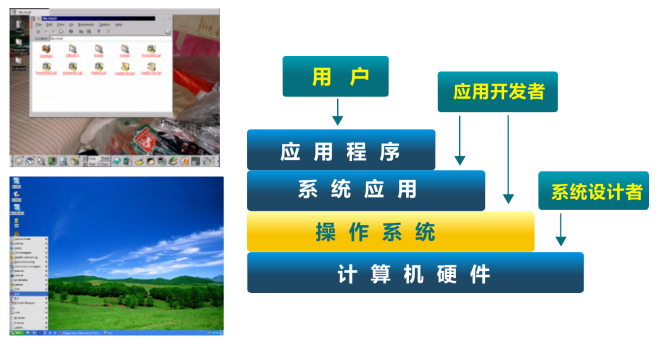
\includegraphics[width=1.\textwidth]{os-position}
			
		\end{column}
		
		\begin{column}{.6\textwidth}
			
	\begin{block}{Interface}
	In computing, an \textbf{\underline{interface }}is a shared boundary across which two or more separate components of a computer system exchange information. [wikipedia]
    \end{block} 
	\LARGE
	What is the OS interface?

		\end{column}
		
		
	\end{columns}
	
	
\end{frame}



%-------------------------------------------------
\begin{frame}[plain]
	\frametitle{Introduction}
	
	
	
	\begin{columns}
		
		\begin{column}{.4\textwidth}
			
			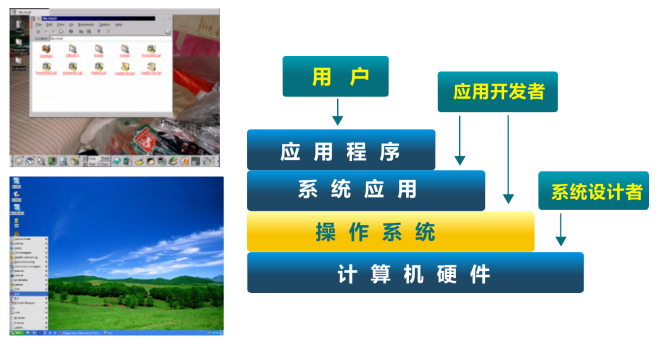
\includegraphics[width=1.\textwidth]{os-position}
			
		\end{column}
		
		\begin{column}{.6\textwidth}
			
			\begin{block}{Application programming interface}
				An \textbf{application programming interface (API) }is a computing interface exposed by a particular software program, library, operating system or internet service, to allow third parties to use the functionality of that software application.
			\end{block} 
			\tiny Fisher, Sharon (1989). "OS/2 EE to Get 3270 Interface Early". 
			
			\normalsize
			\begin{itemize}
				\item POSIX
				\begin{itemize}
					\item Linux,FreeBSD, UNIX, etc.
					
				\end{itemize}
			
				\item Windows API(Win32)
				\begin{itemize}
					\item Windows
				
				\end{itemize}
			\end{itemize}
		\end{column}
		
		
	\end{columns}
	
	
\end{frame}


%-------------------------------------------------
\begin{frame}[plain]
	\frametitle{Introduction}
	
	\begin{center}
	\Huge 
	Implementation of APIs \\
	is the lesser problem
	
	
	\normalsize
	(Performance can be improved later; \\
	bugs are irritating, but can be fixed)
	
	\end{center}

%	How to design a Linux kernel interface,Michael Kerrisk,FOSDEM 2016	
	
\end{frame}


%-------------------------------------------------
\begin{frame}[plain]
	\frametitle{Introduction}
	
	\begin{center}
		\Huge 
		API design is the big problem				
		
	\end{center}
	
	%	How to design a Linux kernel interface,Michael Kerrisk,FOSDEM 2016	
	
\end{frame}

%-------------------------------------------------
\begin{frame}[plain]
	\frametitle{Introduction -- Why is API design a problem?}

	\begin{columns}
	
	\begin{column}{.4\textwidth}
		\centering
		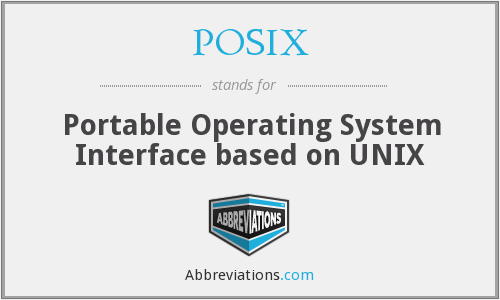
\includegraphics[width=.8\textwidth]{posix}
		
		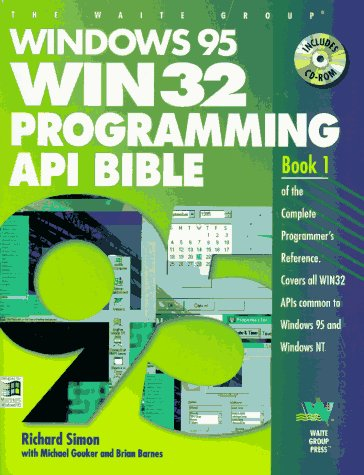
\includegraphics[width=.5\textwidth]{win32}
	\end{column}
	
	\begin{column}{.6\textwidth}
	\large
	\begin{itemize}
	\item Hard to get right
	\item Long-term effect
	\begin{itemize}
		\item Thousands of user-space
		programmers will live with your
		(bad) design for decades
		
	\end{itemize}
	
	\item (Usually) can’t be fixed
	\begin{itemize}
		\item Fix == ABI change
		\item User-space will break
		
	\end{itemize}
	\end{itemize}

\end{column}
\end{columns}

\end{frame}


%-------------------------------------------------
\begin{frame}[plain]
	\frametitle{Windows API -- from the view of software engineering}
	
	
	
	\begin{columns}
		
		\begin{column}{.4\textwidth}
			
			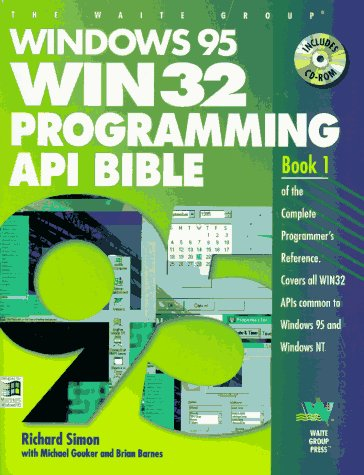
\includegraphics[width=1.\textwidth]{win32}
			
		\end{column}
		
		\begin{column}{.6\textwidth}
			
			Win32 API
			
			\begin{itemize}
				\item Input and output devices: mouse, keyboard, pen, screen,
				printer, and sound.
				
				\item User interface elements: windows, menus, dialogs, input
				widgets, the clipboard, etc.
				
				\item System services: files, memory, hardware, system
				databases, and networking.
				
				\item Graphical elements: bitmaps, fonts, drawing primitives, and 3D graphics rendering, etc.
				
				\item the Microsoft‘s Component Object Model (COM ), OLE, ActiveX,
				
				\item game applications (DirectX 2), etc.
				
				
			\end{itemize}
			
			
		\end{column}
		
		
	\end{columns}
	
	
\end{frame}

%-------------------------------------------------
\begin{frame}[plain]
	\frametitle{Windows API -- from the view of software engineering}
	
	
	
	\begin{columns}
		
		\begin{column}{.4\textwidth}
			
			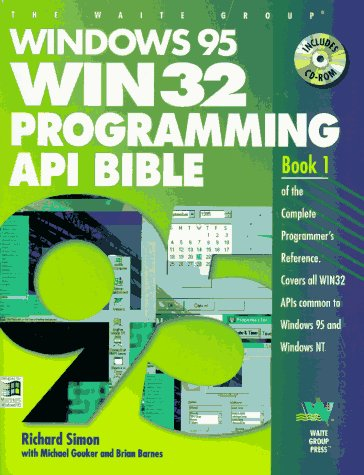
\includegraphics[width=1.\textwidth]{win32}
			
		\end{column}
		
		\begin{column}{.6\textwidth}
			
		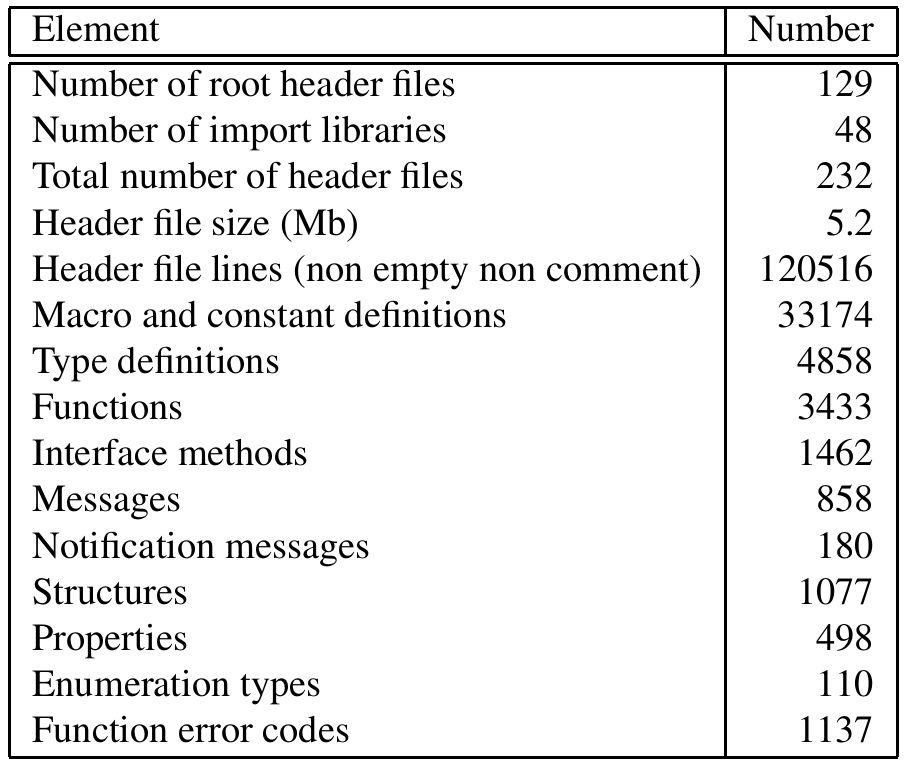
\includegraphics[width=1.\textwidth]{win32api-metrics}
			
		\end{column}
		
		
	\end{columns}
	
	
\end{frame}



%-------------------------------------------------
\begin{frame}[plain]
	\frametitle{Windows API -- from the view of software engineering}
	
	
	
	\begin{columns}
		
		\begin{column}{.4\textwidth}
			
			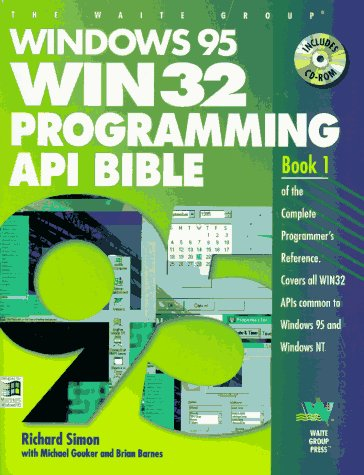
\includegraphics[width=1.\textwidth]{win32}
			
		\end{column}
		
		\begin{column}{.6\textwidth}
		
		Size, Structure, and Implementation of Win32
			
		\begin{itemize}
			\item 9067 API elements (functions, interface methods,
			structures, messages, macros, properties, etc.)
			\item The large size and monolithic nature of the Win32 API
			\item Microsoft’s exclusive control of the API can distort competition and market diversity.
			\item Any formal proof of
			specific properties or the correctness of programs using it is
			an extremely difficult task. 

		\end{itemize}

		\end{column}		
	\end{columns}
	
	
\end{frame}


%-------------------------------------------------
\begin{frame}[plain]
	\frametitle{Windows API -- from the view of software engineering}
	
	
	
	\begin{columns}
		
		\begin{column}{.4\textwidth}
			
			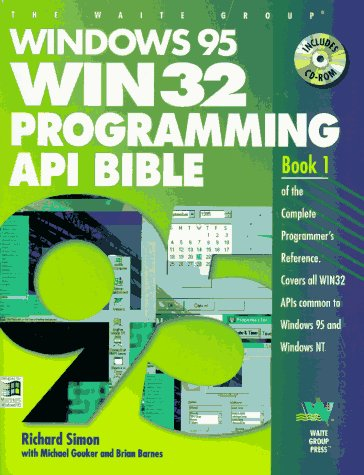
\includegraphics[width=1.\textwidth]{win32}
			
		\end{column}
		
		\begin{column}{.6\textwidth}
			
			Interface of Win32
			
			\begin{itemize}
				\item The provided functions have a complex and non-intuitive
				interface with a number of mode changing flags and exceptions that unnecessarily complicate system application development. 
				\begin{itemize}	
					\item 91 functions that create entities, and the return value inconsistencies across these functions.
					
					\item 131 “extended” functions that perform similar tasks to the original ones. 
					\item e.g. CreateWindowEx has 21 “extended” window
					styles in addition to the 139 styles 
			\end{itemize}
		\end{itemize}
		\end{column}		
	\end{columns}
	
	
\end{frame}


%-------------------------------------------------
\begin{frame}[plain]
	\frametitle{Windows API -- from the view of software engineering}
	
	
	
	\begin{columns}
		
		\begin{column}{.4\textwidth}
			
			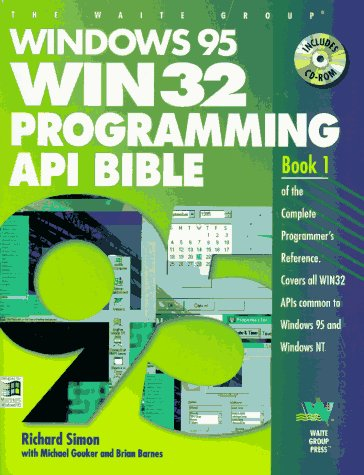
\includegraphics[width=1.\textwidth]{win32}
			
		\end{column}
		
		\begin{column}{.6\textwidth}
			
			Type System Problems in the Interface of Win32
			
			\begin{itemize}
				\item Specifying in a large number
				of cases arguments with minimal type information associated with them. 
				\begin{itemize}	
					\item More than 150 functions pass an argument of type LPVOID or PVOID which is a 	pointer to any type.
					
					\item  even worse abuse of the type system is the use of the LPARAM (32bit) and WPARAM(16bit) type.
				\end{itemize}
			\end{itemize}
		
		EVEV MORE
		\newline \newline
		Namespace Pollution in the Interface of Win32
		\newline \newline
		The functionality of win32 is in a number of cases inconsistent, inadequately documented, or incomplete.  e.g. the spec of 1130 errors.
		
		\end{column}		
	\end{columns}
	
	
\end{frame}
%-------------------------------------------------

%-------------------------------------------------
\end{document}